\documentclass[12pt, twoside]{article}
\documentclass[12pt, twoside]{article}
\usepackage[letterpaper, margin=1in, headsep=0.2in]{geometry}
\setlength{\headheight}{0.6in}
%\usepackage[english]{babel}
\usepackage[utf8]{inputenc}
\usepackage{microtype}
\usepackage{amsmath}
\usepackage{amssymb}
%\usepackage{amsfonts}
\usepackage{siunitx} %units in math. eg 20\milli\meter
\usepackage{yhmath} % for arcs, overparenth command
\usepackage{tikz} %graphics
\usetikzlibrary{quotes, angles}
\usepackage{graphicx} %consider setting \graphicspath{{images/}}
\usepackage{parskip} %no paragraph indent
\usepackage{enumitem}
\usepackage{multicol}
\usepackage{venndiagram}

\usepackage{fancyhdr}
\pagestyle{fancy}
\fancyhf{}
\renewcommand{\headrulewidth}{0pt} % disable the underline of the header
\raggedbottom
\hfuzz=2mm %suppresses overfull box warnings

\usepackage{hyperref}
\usepackage{float}

\title{Algebra 2}
\author{Chris Huson}
\date{May 2024}

\fancyhead[LE]{\thepage}
\fancyhead[RO]{\thepage \\ Name: \hspace{1.5cm} \,\\}
\fancyhead[LO]{BECA/Huson/Algebra 2: Regents Preparation \\* 23 May 2024}

\begin{document}

\subsubsection*{Prep \#16 Polynomials and algebra}
\begin{enumerate}[itemsep=0.5cm]

\item Simplify each expression.
    \begin{multicols}{2}
    \begin{enumerate}[itemsep=0.75cm]
        \item $\displaystyle x^{\frac{2}{3}} \cdot x^{\frac{1}{3}} =$
        \item $\displaystyle x^{\frac{4}{5}} \cdot x^{\frac{6}{5}} =$
        \item $\displaystyle \frac{\sqrt[3]{8x^2}}{\sqrt{16x}} = $
        \item $\displaystyle (x^{\frac{3}{2}}y^3)^2 =$
        \item $\displaystyle (x^{\frac{2}{3}}y^4)^{\frac{1}{2}} =$
        \item $\displaystyle \frac{x^{\frac{3}{4}}}{x^{\frac{1}{4}}} =$
    \end{enumerate}
    \end{multicols} \vspace{0.5cm}

\item Write the expression as a polynomial in standard form.
    \begin{multicols}{2}
    \begin{enumerate}
        \item $(x-3)(x+3)$
        \item $(x+y)(x^2-xy+y^2)$
    \end{enumerate}
    \end{multicols} \vspace{3cm}

\item Simplify each complex expression to the form $a+bi$, with real numbers $a$ and $b$.
    \begin{multicols}{2}
    \begin{enumerate}[itemsep=4cm]
        \item $(2+3i)(3-4i)=$
        \item $(xi-5)^2=$
        \item $(2xi+4)^2=$
        \item $-2i(\sqrt{-3}+4i)-5i^3$
    \end{enumerate}
    \end{multicols} \vspace{3cm}

\newpage
The quadratic formula:
$\displaystyle x = \frac{-b \pm \sqrt{b^2-4ac}}{2a}$

\item Solve each equation. Expression the answer in $a+bi$ form.
    \begin{multicols}{2}
    \begin{enumerate}[itemsep=0.5cm]
        \item $2x^2+5x+8=0$
        \item $3x^2+7x+5=0$
    \end{enumerate}
    \end{multicols} \vspace{5cm}

\item Determine the solution of each equation algebraically.
    \begin{multicols}{2}
    \begin{enumerate}[itemsep=0.5cm]
        \item $\sqrt{3x+7}=x-1$ %June 2023
        \item $\sqrt{4x+1} = 11-x$ %Aug 2022
        %\item $\sqrt{49-10x} + 5 = 2x$ %Jan 2023
        %\item $\sqrt{6-2x} + x = 2(x+15)-9$ %June 2018
        %\item $2x = 6+2\sqrt{x-1}$ %Jan 2024
        %\item $3\sqrt{x} -2x = -5$ %Jan 2019
    \end{enumerate}
    \end{multicols}

\newpage
Geometric Series:
$$S_n = \frac{a_1 - a_1 r^n}{1-r} \text{ where } r \ne 1$$

\item Write a recursive formula for the sequence 16, 8, 0, $-8$, $\ldots$ \vspace{2cm}

\item A sequence is defined by the recursive formula
\begin{align*}
a_1 &= 30 \\
a_{n} &= a_{n-1}+5
\end{align*}
Write an explicit formula for the sequence. \vspace{2cm}


\item The sum of the first $n$ terms of the geometric sequence beginning $1$, $1.5$, $2.25$, $\ldots$ is 171, rounded to \emph{the nearest integer}. Find $n$. \vspace{2cm}

%F.LE.2: Construct a linear or exponential function symbolically given: a graph, a description of the relationship, or two input-output pairs (including from a table).
\item Complete the table for the geometric sequence $a$.
    \begin{center}
    \begin{tabular}{|p{1cm}|p{1cm}|p{1cm}|p{1cm}|p{1cm}|p{1cm}|}
        \hline
        $n$ & 1 & 2 & 3 & 4 & 5 \\
        \hline
        $a_n$ & 100 & 80 & & & \\[0.25cm]
        \hline
    \end{tabular}
    \end{center}
    Model the sequence with an exponential function.


\newpage
\item A survey was conducted to compare the dietary habits of American and Japanese families. Families were asked which they had eaten for dinner most recently, meat or fish. The proportions of each answer are shown in the table below.
    \begin{center}
        \begin{tabular}{|c|c|c|c|}
            \hline
            Nationality & Meat & Fish & Total \\[0.2cm]
            \hline
            Americans & 0.78 & 0.22 & 1.00 \\[0.25cm]
            \hline
            Japanese & 0.43 & 0.57 & 1.00 \\[0.25cm]
            \hline
        \end{tabular}
    \end{center}
    \begin{enumerate}
        \item Does the survey data indicate that Americans and Japanese families have similiar dietary habits? Justify your answer. \vspace{2cm}
        \item 200 American families and 100 Japanese families participated in the survey. Calculate the number of each category of response and enter it in the appropriate cell in the table below. 
        \begin{center}
            \begin{tabular}{|c|p{1.5cm}|p{1.5cm}|c|}
                \hline
                Nationality & \; Meat & \; Fish & Total \\[0.2cm]
                \hline
                Americans & &  & 200 \\[0.25cm]
                \hline
                Japanese & &  & 100 \\[0.25cm]
                \hline
            \end{tabular}
        \end{center}
        \item The survey was conducted in Kansas City (an inland city) and Tokyo (a city on the Pacific Ocean). How might that affect the survey's findings? 
    \end{enumerate} \vspace{3cm}

    \begin{multicols}{2}
\item An exponential function $f(x)$ is graphed.
\begin{enumerate}
    \item Write down an equation for $f(x)$.\vspace{1.5cm}
    \item Find the average rate of change of the function over the interval $0 < x < 4$.
    \vspace{2cm}
\end{enumerate}
    \begin{flushright}
        \begin{tikzpicture}[x=1cm, y=0.1cm, xscale=1.5]
            \draw [thin, color=lightgray, xstep=1cm,ystep=0.5cm] (0,0) grid (4,51);
            \draw [thick, ->] (0,0) -- (+4.3,0) node [below]{$x$};
            \draw [thick, ->] (0,0) -- (0,53) node [right]{$y$};        
            \foreach \x in {1}
                \draw (\x cm,5pt) -- (\x cm,-5pt) node[below] {$\x$};
            \foreach \y in {0,10,...,50}
                \draw[shift={(0,\y)}] (2pt,0pt)--(-2pt,0pt) node[left]{$\y$};
            \draw [thick, ->, smooth,domain=0.:4.2] plot(\x,{15*(3^(\x/4))});
            \fill (0,15) ellipse [x radius=1.33pt, y radius=2pt];
            \fill (4,45) ellipse [x radius=1.33pt, y radius=2pt];
        \end{tikzpicture}
        \end{flushright}
    \end{multicols}
\newpage
%AII-F.LE.2: Construct a linear or exponential function symbolically given: a graph, a description of the relationship, or two input-output pairs (include reading these from a table).

\item A manufacture of portable speakers finds that its profit varies depending on the number of speakers it makes. The profit, $p(x)$, in thousands of dollars as a function of the number of speakers, $x$, in thousands is modeled by $$p(x) = -x^3+7x^2+6x-25$$
\begin{enumerate}
    \item Graph $y=p(x)$, over the interval $0 \leq x \leq 8$ on the set of axes below.
    \item Over the given interval, state the coordinates of the maximum of $p$ rounding all values to the \emph{nearest integer}. Explain what the point means in terms of the number of speakers and profit. \vspace{3cm}
\end{enumerate}
\begin{center}
    \begin{tikzpicture}[yscale=0.1]
        \draw[gray,thin, xstep=1cm,ystep=10cm] (-3,-41) grid (10,80);
        \draw [thick,<->] (-3.5,0)--(10.5,0) node [right] {$x$};
        \draw [thick,<->] (0,-45)--(0,85) node [above] {$y$};
        \foreach \x in {1}
            \draw[thick] (\x cm,50pt) -- (\x cm,-50pt) node[below] {$\x$};
        \foreach \y in {20}
            \draw[thick] (4pt,\y cm)--(-4pt,\y cm) node[left]{$\y$};
        %\draw [thick,<->] plot[smooth, domain=-2.2:8] (\x, {-(\x*\x*\x)+7*(\x*\x)+6*(\x)-25});
    \end{tikzpicture}
    \end{center}

\newpage
\item Over the set of integers, factor the function $f(x) = x^4-5x^2+4$. \vspace{10cm}

\item Given the function $P(x) = x^3-3x^2-2x+4$, find the value of $P(-1)$ and $P(1)$.\\[5cm]
Now identify the correct statement.
\begin{enumerate}
    \item $(x-1)$ is a factor because $P(-1)=2$.
    \item $(x+1)$ is a factor because $P(-1)=2$.
    \item $(x+1)$ is a factor because $P(1)=0$.
    \item $(x-1)$ is a factor because $P(1)=0$.
\end{enumerate}

\newpage
\item An investment of \$4000 earns a continuous interest rate of 8\%. On the axes below, graph the value of the investment $v(t)$ in thousands of dollars versus time $t$ in years. 
\begin{center}
    \begin{tikzpicture}[scale=1]
        \draw[gray,thin] (0,0) grid (10,10);
        \draw [thick,->] (0,0)--(10.5,0) node [right] {$t$};
        \draw [thick,->] (0,0)--(0,10.5) node [above] {$v(t)$};
        \foreach \x in {0,1,...,10}
            \draw (\x cm,5pt) -- (\x cm,-5pt) node[below] {$\x$};
        \foreach \y in {0,1,...,10}
            \draw[shift={(0,\y)}] (2pt,0pt)--(-2pt,0pt) node[left]{$\y$};
    \end{tikzpicture}
    \end{center}
    \begin{enumerate}
        \item Find the value of the investment after 5 years rounding to the \emph{nearest dollar}. \vspace{3cm}
        \item Find the time it will take the investment to double in value, rounded to the \emph{nearest tenth of a year}. 
    \end{enumerate}

\newpage
\item Biologists are studying a new bacterium. They create a culture with 100 of the bacteria and
anticipate that the number of bacteria will double every 30 hours. Write an equation for the
number of bacteria, $B$, in terms of the number of hours, $t$, since the experiment began. %Jan 2020
\vspace{3cm}

\item During the summer, Adam saved \$4000 and Betty saved \$3500. Adam deposited his money in
Bank A at an annual rate of 2.4\% compounded monthly. Betty deposited her money in Bank B at
an annual rate of 4\% compounded quarterly. Write two functions that represent the value of each
account after $t$ years if no other deposits or withdrawals are made, where Adam's account value is represented by $A(t)$, and Betty's by $B(t)$. \\[6cm]
Using technology, determine, to the \emph{nearest tenth} of a year, how long it will take for the two
accounts to have the same amount of money in them. Justify your answer. %Jan 2024

\end{enumerate}
\end{document}

3.OA.7
Fluently multiply and divide within 100, using such as the relationship between multiplication and division. By the end of Grade 3, know from memory all products of two one-digit numbers.
